\chapter[Produto Desenvolvido]{Produto Desenvolvido}
% [Criar um guia de telas e explicação das funcionalidades do protótipo]

\section {Template Projeto C++}

Utilizando um template para projetos C++ (github.com/CaioIcy/CPP\textunderscore Project\textunderscore Template), que serve como base para um projeto em C++ ser compilado através do CMake com o propósito de ser \textit{cross platform}, o Dauphine
está sendo compilado com sucesso.

\begin{figure}[h]
	\centering
	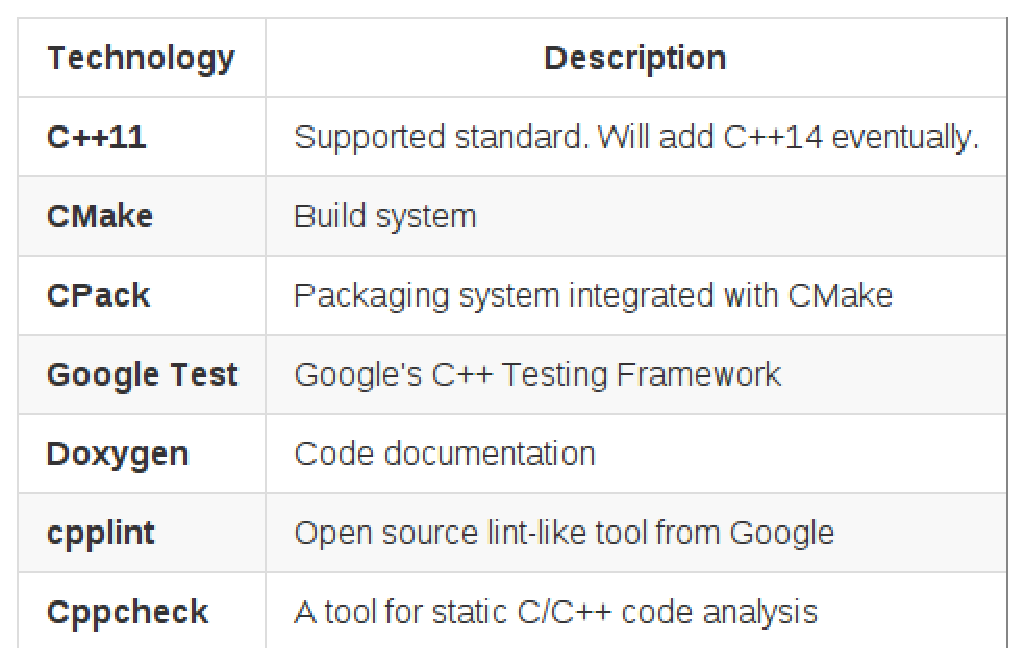
\includegraphics[width=0.6\textwidth]{figuras/cpp_template.eps}
	\caption{Testes sendo executados dentro do Travis CI}
	\label{img:cpp_template}
\end{figure}

\begin{figure}[h]
	\centering
	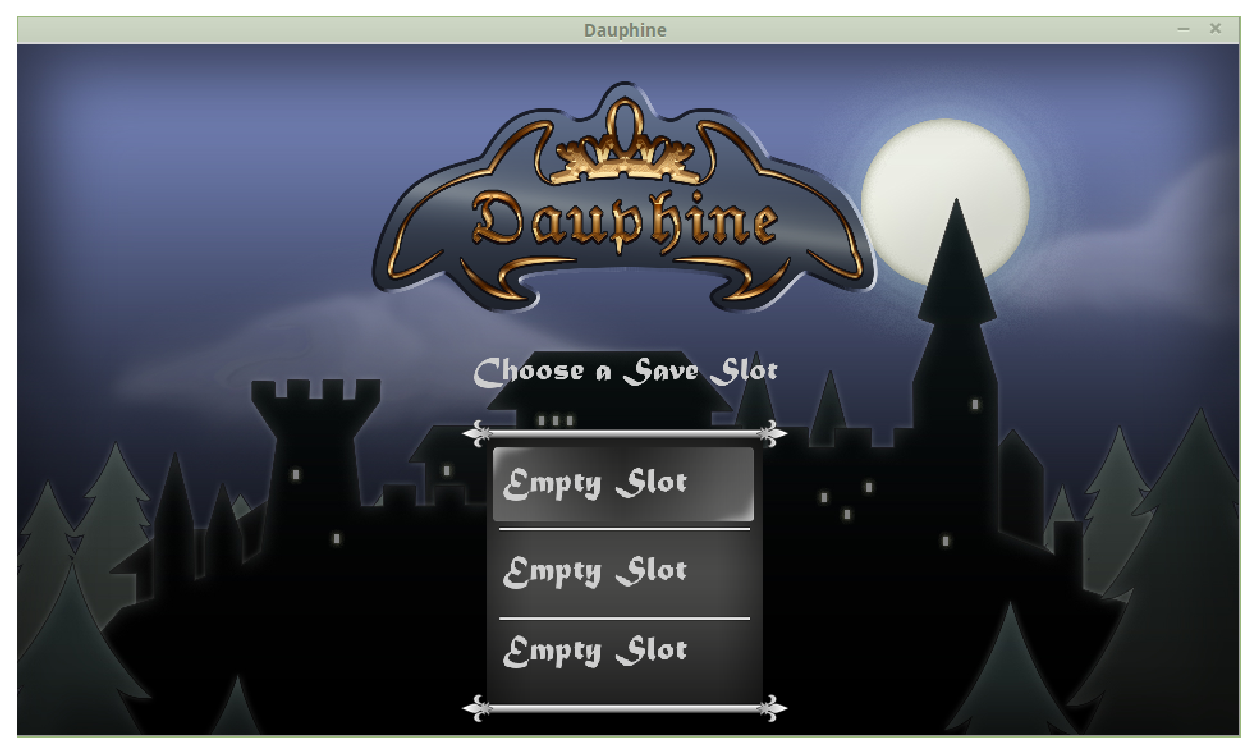
\includegraphics[width=0.8\textwidth]{figuras/vv_dauphine.eps}
	\caption{Menu de Dauphine}
	\label{img:dauphine}
\end{figure}

\begin{figure}[h]
	\centering
	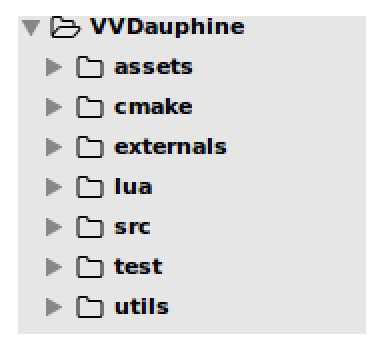
\includegraphics[width=0.4\textwidth]{figuras/vv_cp3t.eps}
	\caption{Estrutura proveniente do template de projetos C++}
	\label{img:cp3t}
\end{figure}

\section {Integração Contínua}

Já com a integração contínua configurada, os testes estão sendo executados a cada commit na branch master.

\begin{figure}[h]
	\centering
	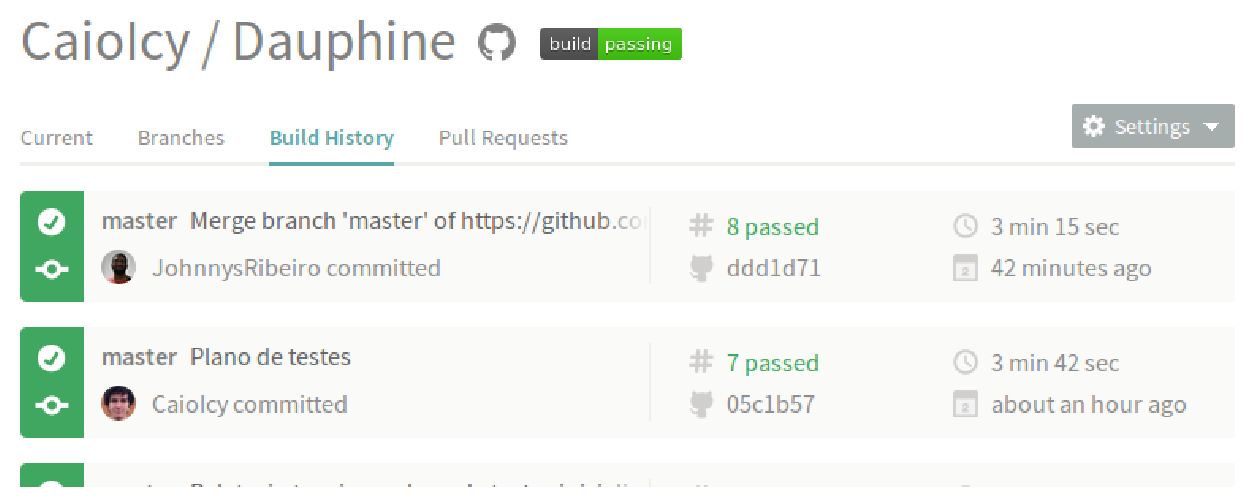
\includegraphics[width=0.8\textwidth]{figuras/vv_travis.eps}
	\caption{Histórico de builds no Travis CI}
	\label{img:travis}
\end{figure}

Os teste desenvolvidos com o framework Google Test, são executados no TravisCI e geram os logs de assertivas.

\newpage

\begin{figure}[h]
	\centering
	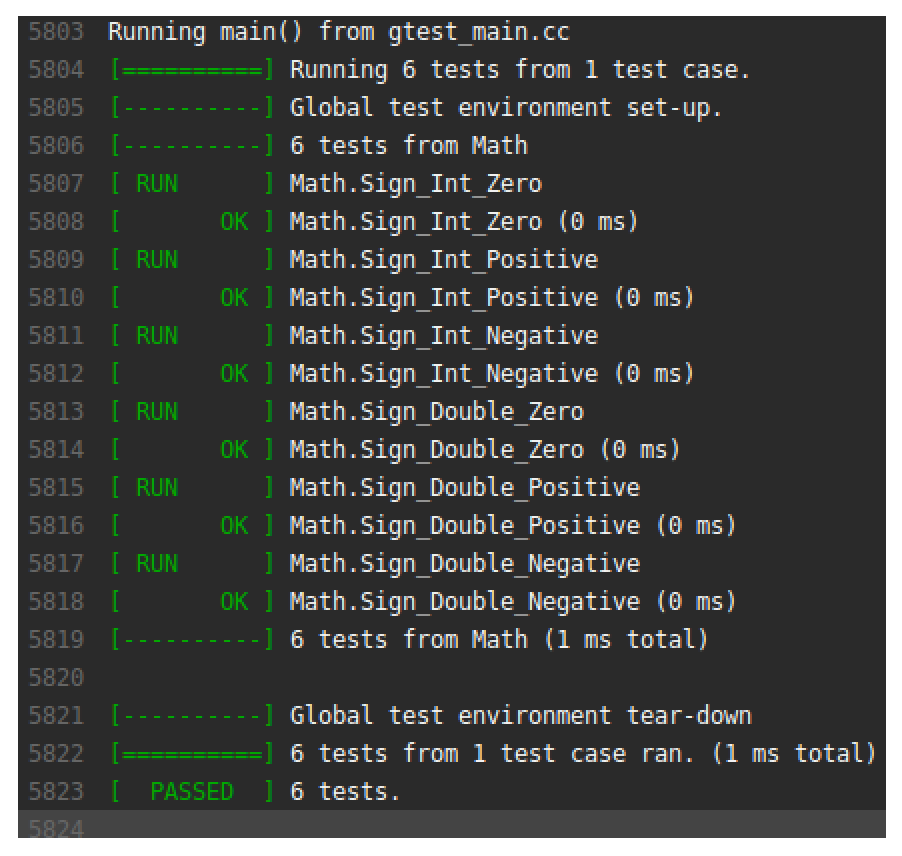
\includegraphics[width=0.6\textwidth]{figuras/vv_travis_tests.eps}
	\caption{Testes sendo executados dentro do Travis CI}
	\label{img:travis_tests}
\end{figure}

\section {Métricas de Código}

As métricas de código tinham como objetivo mapear a evolução da qualidade ao longo das refatorações identificadas pelos testes unitários.

\section {Desenvolvedores Entrevistados}

Com o objetivo de entender as dificuldades de testes unitários automatizados no contexto de jogos, foram contactados 12 desenvolvedores independentes de brasília para responder um questionário sobre testes unitários em jogos.

Foram aplicadas quatro afirmações onde os respondentes as julgariam numa escala de 1 a 5, com 1 sendo "nada" e 5 "muito". As afirmações eram as seguintes:
\begin{itemize}
\item \textit{Você sabe o que são testes unitários}
\item \textit{Teste automatizado facilita o desenvolvimento}
\item \textit{Me sinto confortável/capaz de escrever bons testes unitários}
\item \textit{Na minha empresa/meus projetos de jogos eu faço testes unitários}
\end{itemize}

\begin{figure}[H]
	\centering
	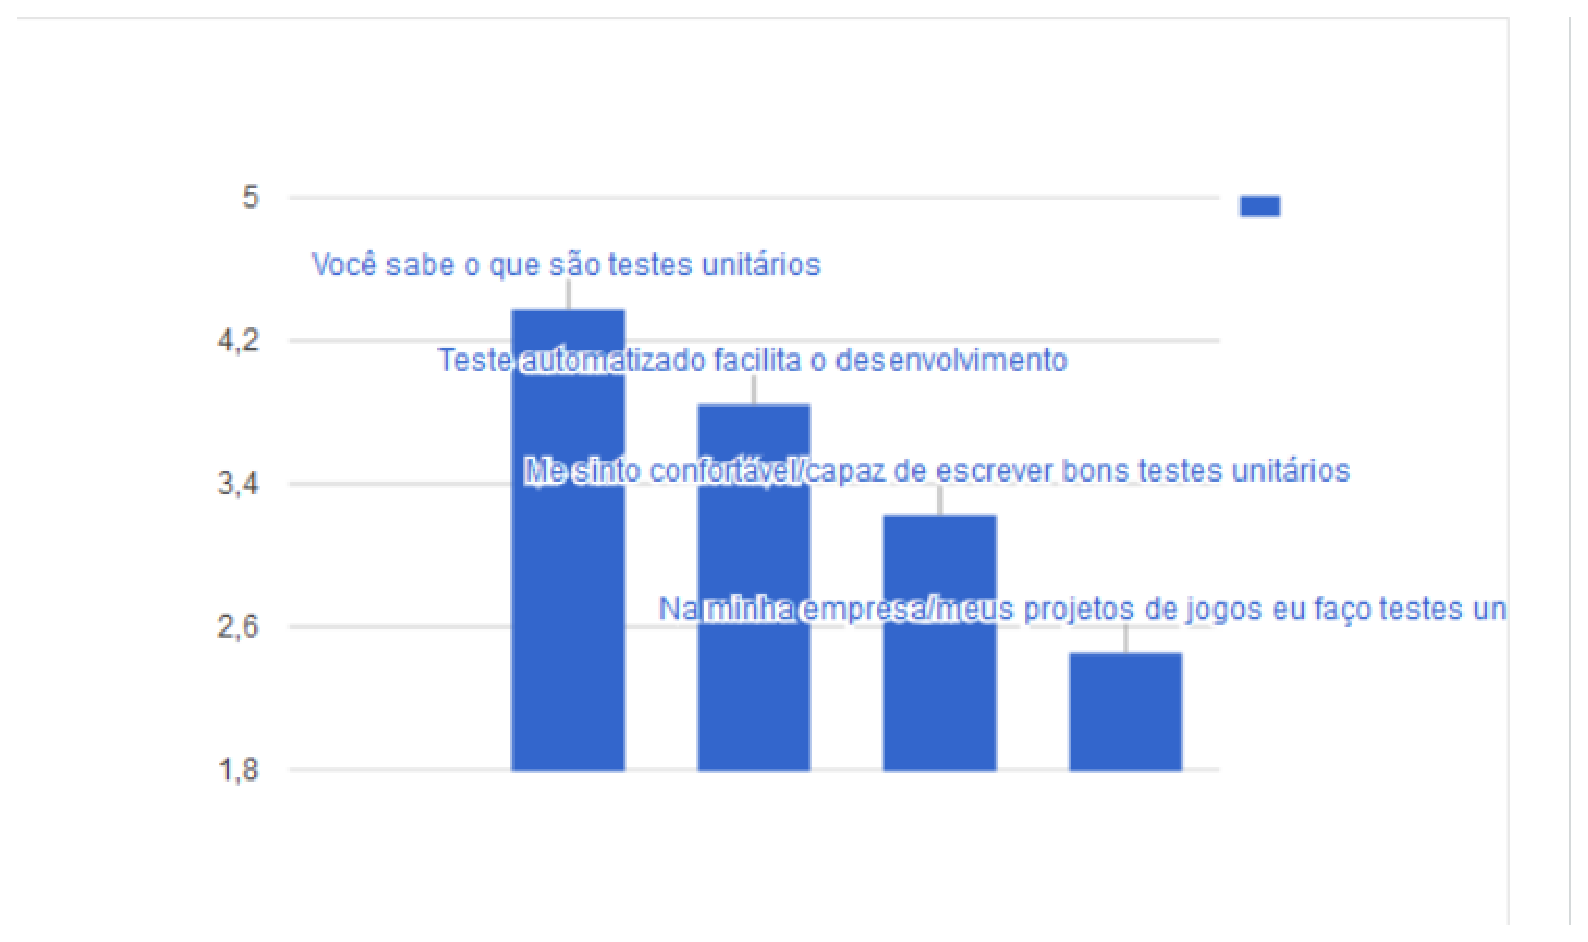
\includegraphics[width=0.6\textwidth]{figuras/questions.eps}
	\caption{Médias dos pontos entrevistados}
	\label{img:questions}
\end{figure}

A partir dos dados levantados viu-se que os desenvolvedores em geral estão cientes da existência de testes unitários, apesar de algumas vezes não terem completo domínio das técnicas de elaboração e implementação de tais testes, levando à conclusões errôneas por parte dos desenvolvedores, como por exemplo entender que deve ser testado apenas a API e não as funcionalidades.

Outro ponto levantado pelos desenvolvedores foi a questão de que os módulos específicos são muito voláteis e por isso os testes iriam sempre mudar junto, aumentando ainda mais o tempo de desenvolvimento do produto.

As médias foram as seguintes:
\begin{itemize}
\item \textbf{4.38}: \textit{Você sabe o que são testes unitários}
\item \textbf{3.84}: \textit{Teste automatizado facilita o desenvolvimento}
\item \textbf{3.23}: \textit{Me sinto confortável/capaz de escrever bons testes unitários}
\item \textbf{2.46}: \textit{Na minha empresa/meus projetos de jogos eu faço testes unitários}
\end{itemize}

O resultado das três primeiras afirmações estão acima da média de \textit{2.5}, e a última está abaixo. Pode ser analisado que os desenvolvedores admitem possuir conhecimento teórico sobre o assunto, porém muitas vezes não aplicam na prática.